\documentclass[11pt]{article}

\usepackage[margin=1in]{geometry}
\usepackage{amsmath,amssymb,amsthm,mathtools}
\usepackage{bm}
\usepackage{graphicx}
\usepackage{booktabs}
\usepackage{array}
\usepackage{xcolor}
\usepackage[colorlinks=true,linkcolor=blue,citecolor=blue,urlcolor=blue]{hyperref}

\graphicspath{{figures/}}

% ----------------------------------------------------------------------
% Notation macros (single source of truth for symbols used throughout)
% ----------------------------------------------------------------------
\newcommand{\R}{\mathbb{R}}
\newcommand{\Z}{\mathbb{Z}}
\newcommand{\simplex}[1]{\Delta^{#1}}
\newcommand{\sites}{\mathcal{S}}
\newcommand{\phenos}{\mathcal{K}}
\newcommand{\states}{\mathcal{X}}
\newcommand{\clones}{\mathcal{C}}
\newcommand{\flatidx}{\iota}              % flattening (site,phenotype) -> index
\newcommand{\Tg}{T^{\mathrm{g}}}          % global transition row
\newcommand{\Tp}{T^{\mathrm{p}}}          % patient transition row
\newcommand{\fdest}{f^{\mathrm{dst}}}     % destination phenotype composition
\newcommand{\ndst}{n^{\mathrm{dst}}}
\newcommand{\nsrc}{n^{\mathrm{src}}}
\newcommand{\Mult}{\mathrm{Multinomial}}
\newcommand{\Dir}{\mathrm{Dirichlet}}
\newcommand{\Gam}{\mathrm{Gamma}}
\newcommand{\mig}{m}                       % migration rate
\newcommand{\tra}{r}                       % phenotype-transition rate
\newcommand{\exg}{g}                       % expansion (growth/death) rate

\title{Estimating T-cell trafficking rates in glioblastoma:\\[2pt]
       \large from clonal tracking to a continuous-time Markov chain}
\author{Nick Ceglia}
\date{\today}

\begin{document}
\maketitle

\noindent
We track T-cell clones across anatomical sites and time in glioblastoma and ask
\emph{at what rates cells move between sites and change phenotype}. We approach
this in three layers, developed in order:
\begin{enumerate}\itemsep2pt
  \item a \textbf{Bayesian phenotype-transition model} that estimates directed,
        per-tissue-pair transition probabilities with patient-level pooling
        (Sec.~\ref{sec:bayes}) --- this is where ``the rates we want'' are made
        precise;
  \item the \textbf{empirical transition matrix} $P$, a model-free estimate of
        the joint (site\,$\times$\,phenotype) dynamics obtained directly from
        clonal tracking (Sec.~\ref{sec:empirical});
  \item the \textbf{continuous-time generator} $Q$ with $P=\exp(Q\,\Delta t)$,
        which factors the dynamics into interpretable \emph{migration},
        \emph{phenotype-transition}, and \emph{expansion} rates
        (Sec.~\ref{sec:ctmc}), with an open-system (birth/death) extension
        (Sec.~\ref{sec:open}).
\end{enumerate}
This section fixes the notation used throughout.

% ======================================================================
\section{Problem setup and definitions}
\label{sec:setup}

\subsection{From cells to tensors}

Everything is built from one tagged object and a binning; each step adds a
single definition.

\begin{enumerate}\itemsep3pt
\item \textbf{Cell.} Every T cell carries five tags: clone $c$ (its TCR$\beta$),
      patient $p$, timepoint $t$, tissue $s$, phenotype $k$.
\item \textbf{Axes.} Cells are sorted on two categorical axes --- tissue
      $\sites=\{\textsf{PBMC},\textsf{CSF},\textsf{TP}\}$ ($S=3$) and phenotype
      ($K=11$). Their product is the \emph{joint state} $x=(s,k)$, with
      $N=SK=33$ values, flattened site-major by $\flatidx(s,k)=sK+k$.
\item \textbf{Bin.} Fix a clone $c$ and time $t$. The bin $(s,k)$ holds one
      number: how many of $c$'s cells are in tissue $s$ with phenotype $k$.
\item \textbf{Count tensor.} Stacking the bins over time gives, \emph{per
      clone}, a 3-D tensor of counts
      \[
        n_c\in\Z_{\ge0}^{\,T\times S\times K},\qquad
        n_c[t,s,k]=\#\{\text{cells of }c\text{ at time }t\text{ in bin }(s,k)\}.
      \]
      Picture $T=6$ time-slices, each an $S\times K=3\times11$ grid of $33$ bins
      (over all clones, a 4-D array $|\clones|\times T\times S\times K$).
      Flattening $(s,k)\!\to\! x$ makes each slice a length-$N$ vector
      $n_{c,t}\in\Z_{\ge0}^{N}$.
\item \textbf{Clone total.} $N_{c,t}=\sum_x n_{c,t}(x)$ is how many cells of $c$
      were seen at $t$. Keep a slice only if $N_{c,t}\ge2$.
\item \textbf{State vector.} Normalising a slice says \emph{where the clone's
      mass sits}: $\;v_{c,t}=n_{c,t}/N_{c,t}\in\simplex{N-1}$, a distribution
      over the $33$ states (sums to $1$).
\item \textbf{Observation.} A retained consecutive pair is one datum:
      $(v_{c,t},\,v_{c,t+1})$ with weight $w_{c,t}=N_{c,t}+N_{c,t+1}$. Steps are
      one interval, $\Delta t=1$ (timepoint index, not days), so all rates are
      \textbf{per interval}. The $M$ pairs stack into
      $\mathbf{S},\mathbf{D}\in\R^{M\times N}$ --- the input to $P$
      (Sec.~\ref{sec:empirical}).
\end{enumerate}

\subsection{The Bayesian reduction}

The Bayesian model (Sec.~\ref{sec:bayes}) looks at one \emph{directed} tissue
pair $(a\!\to\! b)$, $a,b\in\sites$, and one lineage $\ell$ ($K_\ell$
phenotypes: $7$ for CD8, $4$ for CD4; cross-lineage clones dropped). From a
clone's count tensor it takes two phenotype vectors --- the profile in the
source tissue and the counts in the destination tissue one step later,
\[
  \nsrc_c(k)=n_c[t,a,k],\qquad
  \ndst_c(k)=n_c[t{+}1,b,k]\ \in\Z_{\ge0}^{K_\ell},
\]
then forms the (smoothed, fixed) source distribution
$\theta_c\propto\nsrc_c+0.1\in\simplex{K_\ell-1}$ and the destination size
$N_c=\sum_k\ndst_c(k)$. Learning how $\theta_c$ maps to $\ndst_c$ folds
migration and phenotype change into one matrix --- which the CTMC later pulls
apart.

\subsection{Notation summary}

Table~\ref{tab:notation} collects every symbol; objects defined in later
sections ($P$, $Q$, and the three rate families) are listed with forward
references.

\begin{table}[h]
\centering
\small
\renewcommand{\arraystretch}{1.25}
\begin{tabular}{@{}l l l@{}}
\toprule
\textbf{Symbol} & \textbf{Meaning} & \textbf{Notes / value} \\
\midrule
\multicolumn{3}{@{}l}{\emph{Indices and sets}}\\
$s,a,b\in\sites$            & tissue / site                    & $\{\textsf{PBMC},\textsf{CSF},\textsf{TP}\}$, $S=3$\\
$k,u,v\in\phenos$          & phenotype                        & $K=11$ joint; $K_\ell$ per lineage\\
$\ell\in\{\textsf{CD8},\textsf{CD4}\}$ & lineage              & switching clones removed\\
$x=(s,k)\in\states$        & joint state                      & $N=SK=33$\\
$\flatidx(s,k)=sK+k$       & flat index (site-major)          & $0,\dots,N-1$\\
$c\in\clones$              & clone (TCR$\beta$)               & lineage tracer\\
$p\in\{1,\dots,P\}$        & patient                          & hierarchical grouping\\
$t\in\{1,\dots,T\}$        & timepoint                        & $T=6$; pairs $(t,t{+}1)$, $\Delta t=1$\\
$(a\!\to\! b)$             & directed tissue pair             & $a,b\in\sites$; Sec.~\ref{sec:bayes}\\
\addlinespace
\multicolumn{3}{@{}l}{\emph{Observed / fixed data}}\\
$n_{c,t}(s,k)$             & cells of clone $c$ at $t$ in $(s,k)$ & \\
$N_{c,t}=\sum n_{c,t}$     & clone total at $t$               & retained if $\ge 2$\\
$v_{c,t}\in\simplex{N-1}$  & fractional state vector          & $v=n_{c,t}/N_{c,t}$\\
$\nsrc_c,\ndst_c\in\Z_{\ge0}^{K_\ell}$ & clone phenotype counts in tissue $a$ / $b$ & \\
$\theta_c\in\simplex{K_\ell-1}$ & source phenotype distribution & $\theta_c\propto \nsrc_c+0.1$\\
$N_c=\sum_v \ndst_c(v)$    & destination cell total           & Multinomial size\\
$\fdest\in\simplex{K_\ell-1}$ & destination phenotype composition in $b$ & prior centre\\
\addlinespace
\multicolumn{3}{@{}l}{\emph{Parameters and estimands}}\\
$\Tg_{k},\,T_{k}\in\simplex{K_\ell-1}$ & global / pooled transition row & Sec.~\ref{sec:bayes}\\
$\Tp_{p,k}\in\simplex{K_\ell-1}$ & patient-$p$ transition row     & Sec.~\ref{sec:bayes}\\
$\kappa$                   & global$\to$patient pooling concentration & $\Gam(5,1)$\\
$\alpha\in\R^{K_\ell}$     & Dirichlet prior concentration    & $\alpha=K_\ell\,\fdest$, floored at $0.5$\\
$\pi_c=\theta_c\,\Tp_{p(c)}$ & expected destination distribution & deterministic\\
$P\in\R^{N\times N}$       & empirical transition matrix      & row-stochastic; Sec.~\ref{sec:empirical}\\
$Q\in\R^{N\times N}$       & CTMC generator                   & $P=\exp(Q\Delta t)$; Sec.~\ref{sec:ctmc}\\
$\mig^{(k)}_{a\to b}$      & migration rate (site $a\!\to\! b$, phenotype $k$ fixed) & Sec.~\ref{sec:ctmc}\\
$\tra^{(s)}_{u\to v}$      & phenotype-transition rate ($u\!\to\! v$, site $s$ fixed) & Sec.~\ref{sec:ctmc}\\
$\exg_{s,k}$               & expansion (growth $+$ / death $-$) rate & Sec.~\ref{sec:open}\\
\bottomrule
\end{tabular}
\caption{Master notation. The Bayesian model (Sec.~\ref{sec:bayes}) operates on
the phenotype-only, per-lineage space ($K_\ell$); the empirical matrix and
generator (Secs.~\ref{sec:empirical}--\ref{sec:open}) operate on the full joint
space ($N=33$).}
\label{tab:notation}
\end{table}

\subsection{The basic model at a glance}

Figure~\ref{fig:plate} is the generative skeleton of the Bayesian model
(Sec.~\ref{sec:bayes}), shown here to anchor the symbols above. Reading
left-to-right is the generative flow: a fixed prior $\alpha$ and a latent pooling
strength $\kappa$ shape global transition rows $\Tg_k$, which are sharpened into
patient-specific rows $\Tp_{p,k}$; each clone's observed source profile
$\theta_c$ is pushed through its patient's matrix to predict its observed
destination counts $\ndst_c$.

\begin{figure}[h]
\centering
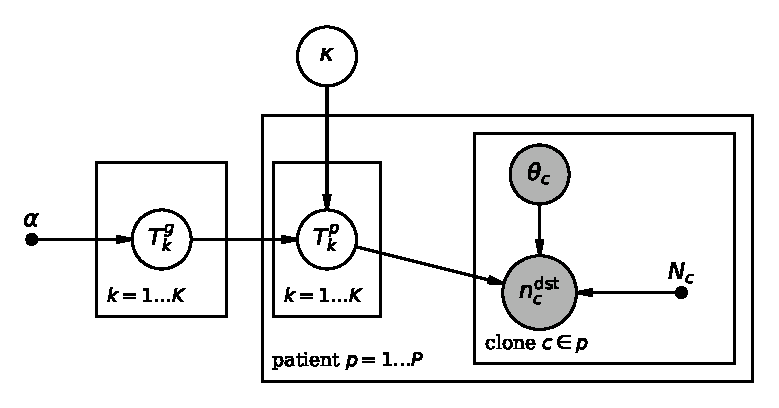
\includegraphics[width=0.85\textwidth]{plate_basic.pdf}
\caption{Plate diagram of the basic (per directed pair $a\!\to\! b$, per
lineage $\ell$) generative model. Open circles are latent (estimated); shaded
circles are observed data, solid dots are fixed constants.}
\label{fig:plate}
\end{figure}

\noindent\textbf{Variables in Figure~\ref{fig:plate}.}
\begin{description}\itemsep1pt
  \item[$\alpha$ \normalfont(fixed)] Dirichlet prior concentration, $\alpha=K_\ell\,\fdest$
        (floored at $0.5$); centres the prior on the destination composition.
  \item[$\kappa$ \normalfont(latent)] global$\to$patient pooling strength,
        $\kappa\sim\Gam(5,1)$; larger $\kappa$ shrinks patients toward $\Tg$.
  \item[$\Tg_k$ \normalfont(latent)] global transition row for source phenotype $k$,
        $\Tg_k\sim\Dir(\alpha)$ --- the population-level estimand.
  \item[$\Tp_k$ \normalfont(latent)] patient-$p$ transition row,
        $\Tp_k\sim\Dir(\kappa\,\Tg_k)$.
  \item[$\theta_c$ \normalfont(observed)] clone source phenotype distribution in source tissue $a$.
  \item[$\ndst_c$ \normalfont(observed)] clone destination counts in destination tissue $b$,
        $\ndst_c\sim\Mult(N_c,\pi_c)$ with $\pi_c=\theta_c\,\Tp_{p(c)}$.
  \item[$N_c$ \normalfont(fixed)] destination cell total (Multinomial size).
\end{description}
The deterministic mean $\pi_c=\theta_c\,\Tp_{p(c)}$ is folded into the two edges
entering $\ndst_c$.
\emph{Figure generated by \texttt{docs/figures/plate\_basic.py}.}

% ======================================================================
\section{The Bayesian phenotype-transition model}
\label{sec:bayes}
\emph{[To be developed next: the full generative model, prior construction from
$\fdest$, the hierarchical pooling via $\kappa$, the multinomial likelihood, and
SVI inference.]}

\section{The empirical transition matrix \texorpdfstring{$P$}{P}}
\label{sec:empirical}
\emph{[To be developed: clone-pair construction, the weighted least-squares
estimator for $P$, and its interpretation.]}

\section{From \texorpdfstring{$P$}{P} to the continuous-time generator \texorpdfstring{$Q$}{Q}}
\label{sec:ctmc}
\emph{[To be developed: the closed CTMC, the migration/transition factorisation
of $Q$, and the two estimators (matrix log and structured Frobenius fit).]}

\section{Open-system extension: birth and death}
\label{sec:open}
\emph{[To be developed: the augmented state with an unobserved compartment, and
the exit/entry/expansion rates.]}

\end{document}
